Para encapsular las funciones y los procedimientos necesarios para implementar la funcionalidad del proyecto, hemos realizado 4 divisiones.


\section{Clientes}
En este paquete, encontraremos funcionalidades que actuarán sobre los datos de los clientes, tales como insertar, modificar, eliminar un único cliente o todos al mismo tiempo, listar un cliente dado su número identificador, listar todos los clientes registrados y por último, listar las reservas de un cliente.

\begin{figure}[ht]
    \centering
    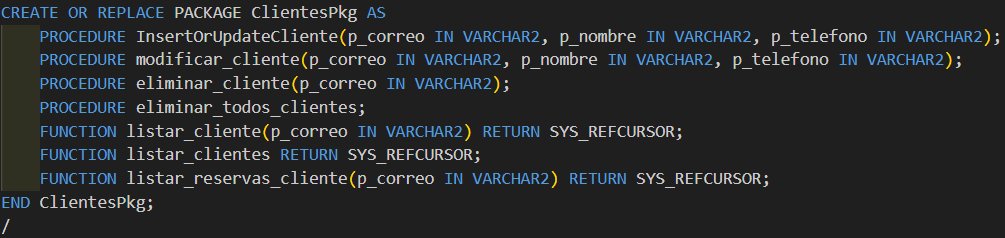
\includegraphics[width=0.7\linewidth]{documentation//apartados//paquetes/paquete-clientes.png}
    \caption{Paquete de Clientes.}
\end{figure}

\section{Películas}
Las películas tendrán funciones para ser eliminadas (ya sea por ID o de forma masiva), listadas (de la misma forma que la eliminación), y para obtener la película que más eligen los usuarios.

\begin{figure}[ht]
    \centering
    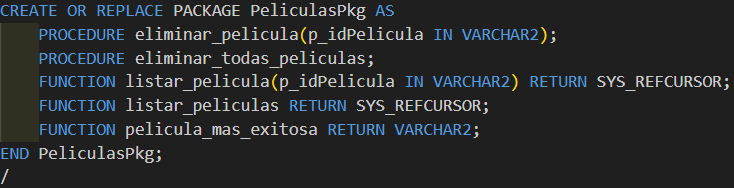
\includegraphics[width=0.7\linewidth]{documentation//apartados//paquetes/paquete-peliculas.png}
    \caption{Paquete de películas.}
\end{figure}

\section{Reservas}
En el caso de las reservas, podrán ser eliminadas mediante un identificador, listadas por ID o en masa, creadas y además, su paquete contendrá una función para calcular el importe total que el usuario ha de abonar, y otra función que devolverá el menú más solicitado por los clientes.


\begin{figure}[ht]
    \centering
    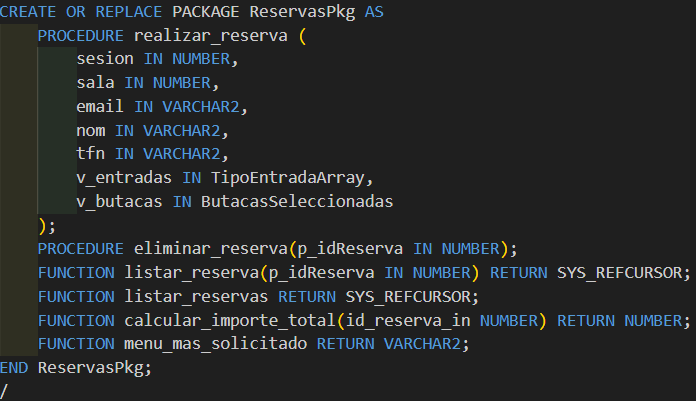
\includegraphics[width=0.7\linewidth]{documentation//apartados//paquetes/paquete-reservas.png}
    \caption{Paquete de reservas.}
\end{figure}

\newpage

\section{Sesiones}
Por último, el paquete referente a las sesiones contendrá funciones para eliminarlas (por ID, por película o en masa), calcular las butacas libres de una sesión, devolver sesiones (con butacas libres, por ID o por película y fecha), y una función que devolverá aquellas butacas que ya estén ocupadas.

\begin{figure}[ht]
    \centering
    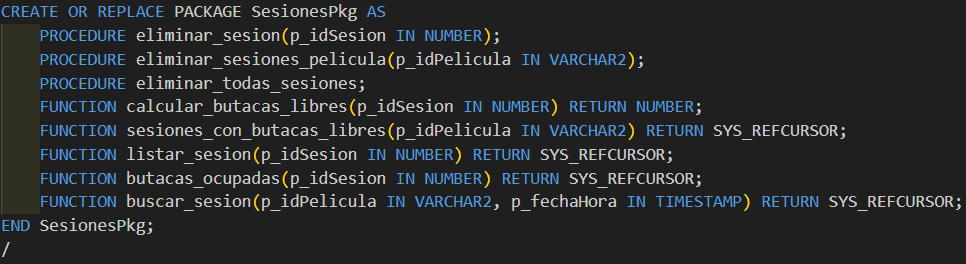
\includegraphics[width=0.7\linewidth]{documentation//apartados//paquetes/paquete-sesiones.png}
    \caption{Paquete de sesiones.}
\end{figure}